\newcommand{\lc}{LC}
\newcommand{\ta}{TA}
\newcommand{\smc}{SMC}
\newcommand{\kcore}{k_{core}}
\newcommand{\kmesh}{k_{mesh}}
\newcommand{\kram}{k_{ram}}

\chapter{\MMSCC: A Coherent and Managed Runtime for ML on the SCC}
\label{chap:aneris}

In this chapter, we describe \MMSCC, an extension of \MM that provides a
coherent address space on the SCC, optimizing for the SCC's memory hierarchy.
We begin with a \emph{local collector}\footnote{Other terms have been used in
the literature to indicate similar heap designs, notably private nursery, local
heap collector, thread-local or thread-specific heap, and on-the-fly
collection.} (\lc) design~\cite{} that partitions the heap into local heaps on
each core and a shared heap for cross-core communication. However, we observe
that the cost of memory barriers utilized in preserving the heap invariants
have significant costs. To eliminitate theses costs, we propose a new GC design
(\ta) that utilizes the ample concurrency offered by our programming model
combined with a dynamic shape analysis to eliminate some of the GC overheads.
This naturally leads to a GC design that focuses on
\emph{procrastination}~\cite{mmgc}, delaying writes that would necessitate
establishing forwarding pointers until a GC, where there is no longer a need
for such pointers. The GC leverages the mostly functional nature of ACML
programs and a new object property called \emph{cleanliness}, which enables a
broad class of objects to be moved from a local to a shared heap without
requiring a full traversal of the local heap to fix existing references;
cleanliness enables an important optimization that achieves the effect of
procrastination without actually having to initiate a thread stall. Our final
design (\smc) integrates SCC's support for software-managed cache coherence
into the extant memory barriers to improve the design further.

We begin by discussing in detail the architecture and programming model of the
SCC, which serves as our prototype non cache coherent architecture. However,
the use of SCC by no means restricts the applicability of our ideas to other
scalable manycore architectures~\cite{mmgc}.

\section{The Intel Single-chip Cloud Computer}

\begin{figure}
\begin{center}
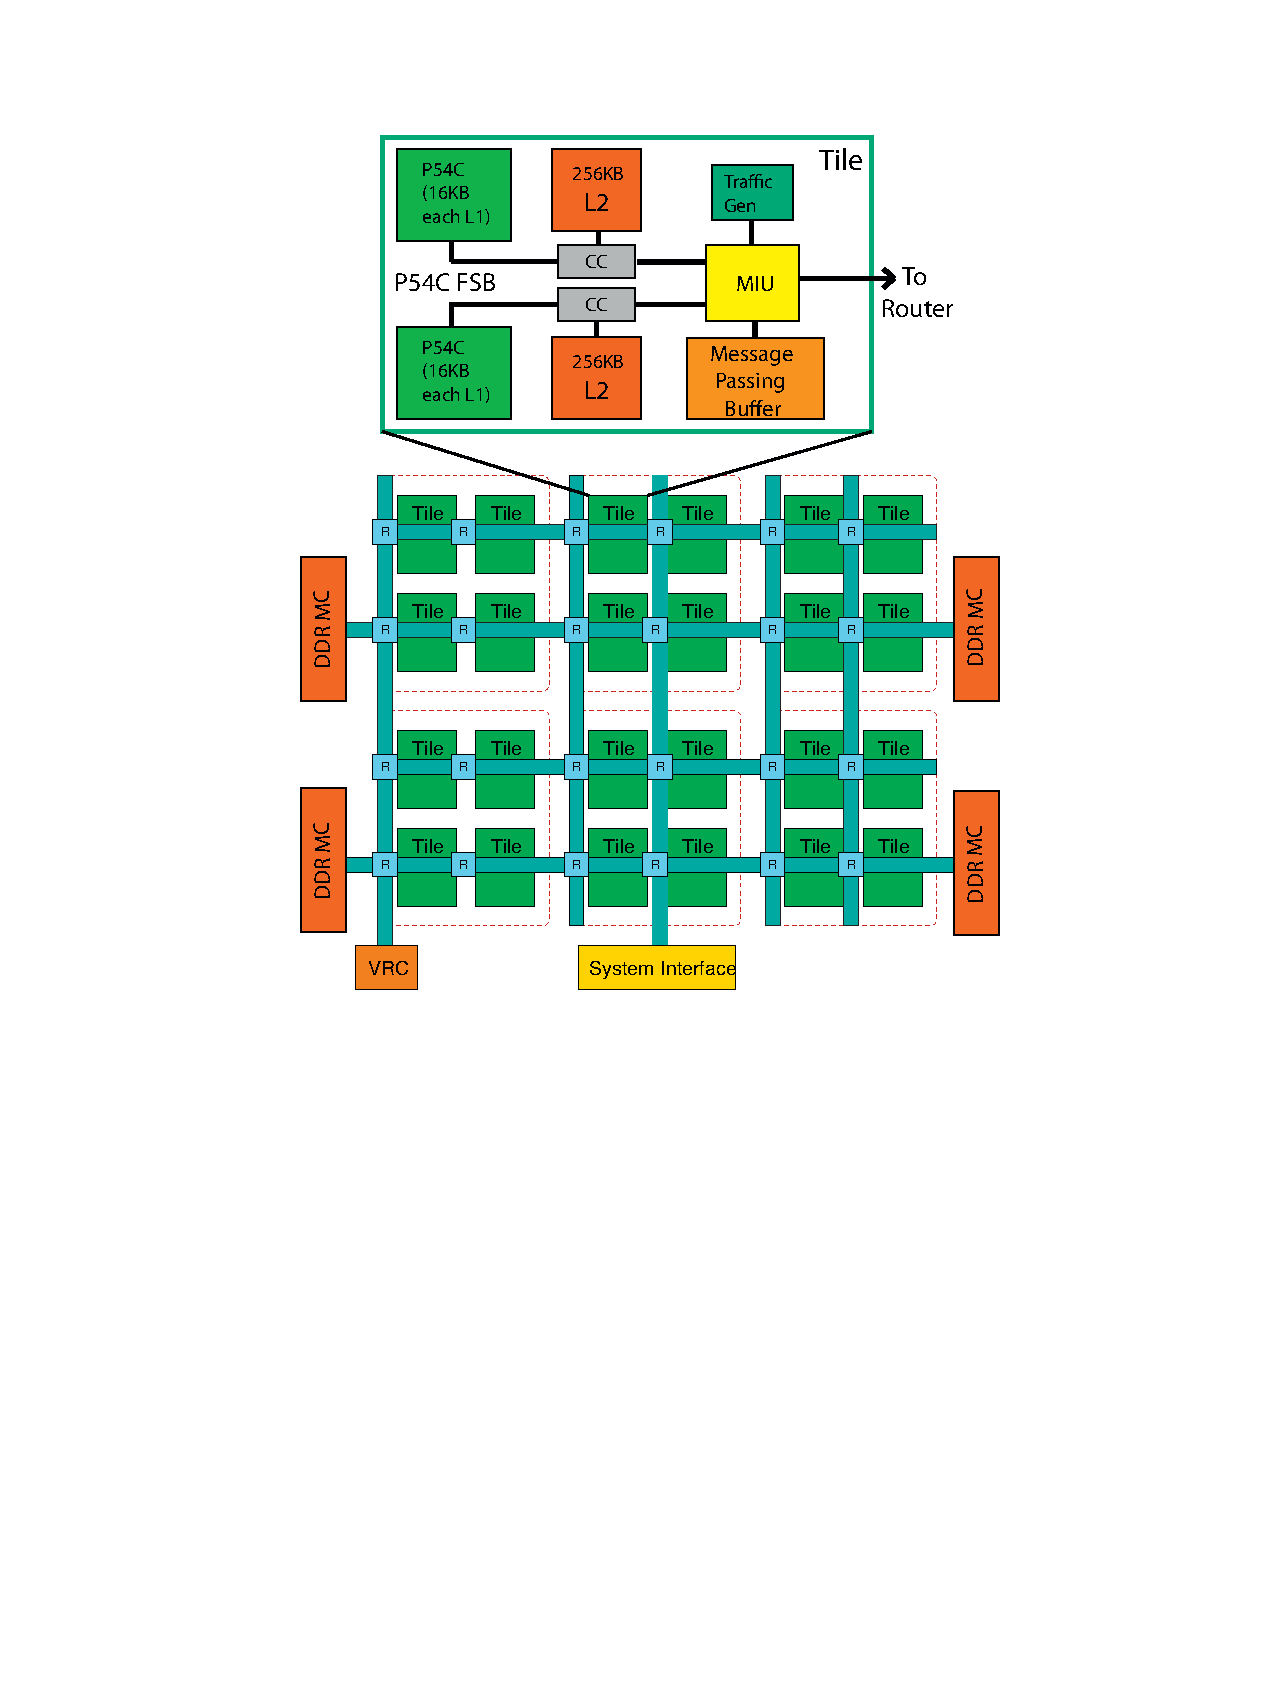
\includegraphics{Figures/SCC.pdf}
\end{center}
\caption{The architecture of the Intel SCC processor}
\label{fig:scc}
\end{figure}

Intel SCC~\cite{Mattson2010} (Figure~\ref{fig:scc}) is a many-core processor
with 48 P54C cores on a single chip, grouped as 24 tiles, organized in a 4
$\times$ 6 mesh network with a bisection bandwidth of 256 Gb/s. The most
interesting aspect of the SCC architecure is the complete lack of cache
coherence between the cores, and the presence of fast on-die message-passing
network interface. The 24 tiles on the chip are divinded into 4 quadrants, and
each quadrant is connected to a DDR3 memory controller. Each core has 16KB of
private L1 instruction and data caches, and 256 KB of L2 cache shared with the
other core on the same tile.

In addition, each tile has a 16KB message-passing buffer (MPB) used for
message-passing between the cores. The message passing buffers are the only
caches that are accessible across all of the cores. The data used in on-chip
communication is read from MPB, cached in L1 cache, but bypasses the L2 cache.
The cache uses no-allocate policy on writes, and L1 cache incorporates a
write-combine buffer. According to the processor
specifications~\cite{Mattson2010}, the read latencies in this architecure are:

\begin{mathpar}
\begin{array}{rcl}
\textrm{LocalMPB} & = & 45~\kcore + 8~\kmesh \\
\textrm{RemoteMPB} & = & 45~\kcore + 4*n*2~\kmesh \\
\textrm{DRAM} & = & 40~\kcore + 4*n*2~\kmesh + 46~\kram
\end{array}
\end{mathpar}

\noindent where $\kcore$, $\kmesh$ and $\kram$ are the cycles of core, mesh
network and memory respectively. In our experimental setup, where 6 tiles share
a memory controller, the number of hops n to the memory controller could be $0
< n \le 8$. Hence, the DRAM accesses are far more expensive than the MPBs. Each
core additionally has a test and set register that is accessible from all other
cores. The SCC uses 32-bit Pentium cores. A programmable, software-managed
Look-Up Table (LUT) provides a means for implementing hybrid private and shared
address spaces in the system.

\subsection{Software System}

From the programmer's point of view, SCC resembles a cluster of nodes, with
portions of memory shared between the cores. Each core runs a linux kernel
image, and does not share any operating system services with the other cores.
Since SCC does not provide harware cache coherence, it provides software
support for managing coherence. First, SCC provides support for tagging a
specific virtual address space as shared across all of the cores. Caching can
also be selectively enabled on this address space; SCC tags this address space
as having message passing buffer type (MPBT).

Data typed as MPBT bypass L2 and go directly to L1. SCC also provides a
special, 1-cycle instruction called \cf{CL1INVMB} that marks all data of type
MPBT as invalid L1 lines. In addition, special 1-cycle instructions are
provided to flush (\cf{INVFLUSH}) and invalidate (\cf{INV}) L1 cache data.
Since the cores use write-combine buffers, a correct flushing procedure should
also flush the write-combine buffers. SCC does not provide primitive support
for this purpose, but write-combine buffers can easily be flushed in software
by perfoming a series of dummy writes to distinct memory locations, which fills
the buffer and flushes any previous writes. Typically, a programmer works with
release consistency in order to utilize cached shared virtual memory. Let us
assume that a core issues a \cf{smcAcquire()} to fetch changes from other cores
and issues \cf{smcRelease()} to publish its updates.

SCC's software stack also includes cross-core message-passing libraries
implemented over the MPBs, including RCCE~\cite{Mattson2010} and
RCKMPI~\cite{Urena2011}. RCCE is optimized for SPMD~\cite{} programming model,
where the program is structured in such a way that the sender and the receiver
ideally arrive at the communication point at the same time. The sender writes
the message to the MPB, while the receiver busy waits (invalidating its cache
every iteration to fetch recent writes), waiting for a special flag value to be
written along with the message. After the sender writes the flag, the receiver
reads the message into its private memory, while the sender busy waits (also
invalidating its cache every iteration). Finally, the receiver writes a
completion flag, which concludes the message transfer.

It is worthwhile pointing out that RCCE uses just the MPBs, while RCKMPI uses
MPBs for small messages (less than 8KB --- the maximum message size that would
fully fit in the MPB) and the DRAM for larger messages. Despite having a higher
bandwidth and lower latency, the synchronization costs involved in transferring
a large multi-part message over the MPB overweighs the benefits.

\section{Local collector design}

Splitting a program heap among a set of cores is a useful technique to exploit
available parallelism on scalable multicore platforms: each core can allocate,
collect, and access data locally, moving objects to a global, shared heap only
when they are accessed by threads executing on different cores. This design
allows local heaps to be collected independently, with coordination required
only for global heap collection. In contrast, stop-the-world collectors need a
global synchronization for every collection.

\begin{figure}
\centering
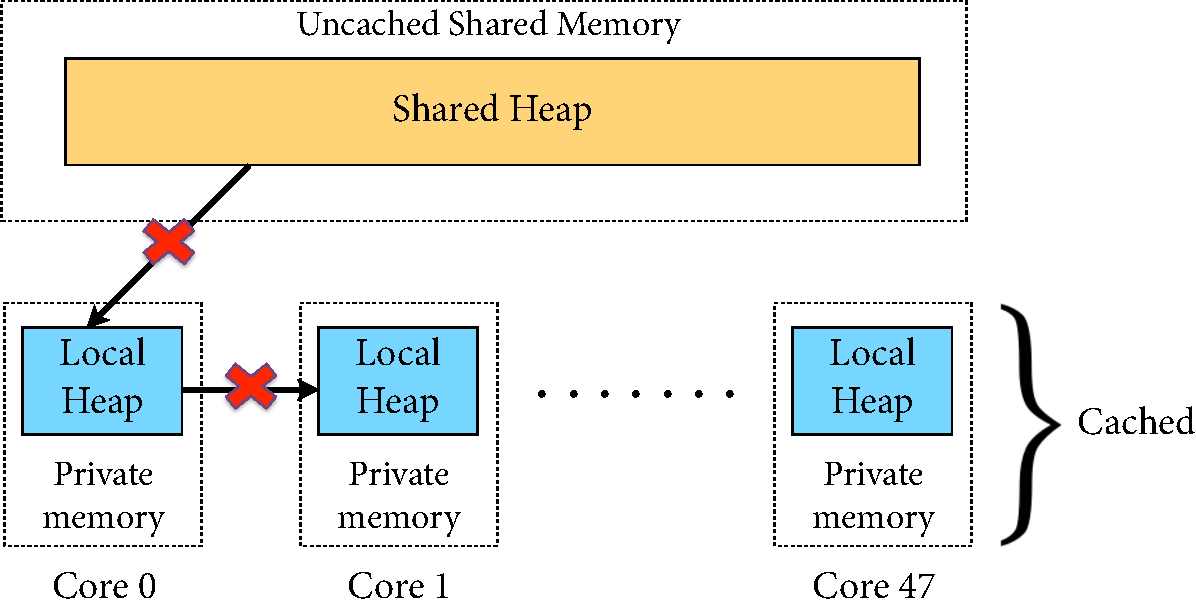
\includegraphics[scale=0.75]{Figures/LocalCollector.pdf}
\caption{Local collector heap organization for the SCC}
\label{fig:lc}
\end{figure}

Our local collector design for the SCC is shown in Figure~\ref{fig:lc}.
